\section{Math and Physics preliminaries} 
Two basic operations in vector algebra are presented below, which are the dot product and the cross product. 
\begin{align}
	\label{dot product}
	\vec{A} \cdot \vec{B} &= 
		\begin{bmatrix}
			a_{x} & a_{y} & a_{z}
		\end{bmatrix} 
		\begin{bmatrix}
			b_{x}\\
			b_{y}\\
			b_{z}
		\end{bmatrix} = S\\	
	\label{cross product}
	\vec{A} \times \vec{B} &= 
		\begin{bmatrix}
			a_{y}b_{z} - b_{y}a_{z}\\
			b_{x}a_{z} - a_{x}b_{z}\\
			a_{x}b_{y} - b_{x}a_{y}
		\end{bmatrix} = \vec{V} 
\end{align}	
$\vec{A}, \vec{B}$ are vectors that live in 3-dimensions, from \autoref{dot product} we find that two vectors produce a scalar. While from \autoref{cross product}, we find that two vectors produce another, third vector that is orthogonal to the first two ($\vec{V} \perp \vec{A}, \vec{B}$). We also have to recall that a dot product in \autoref{dot product} represents a projection of the first vector onto the second vector. From these pieces of information, we can also derive the following. 
\begin{align}
	\label{cross cross} 
	\vec{A} \times \vec{A} &= 0\\
	\label{dot cross}
	\vec{A} \cdot \Big[ \vec{A} \times \vec{B} \Big] &= 0
\end{align}
Clearly, projecting a vector onto another vector that is orthogonal to it would lead to the zero vector. We can further write the following identities. 
\begin{align}
	\vec{A} \cdot \Big[ \vec{B} \times \vec{C} \Big] &= \Big[\vec{A} \times \vec{B} \Big] \cdot C\\
	\vec{A} \times \Big[\vec{B} \times \vec{C} \Big] &= \vec{B}(\vec{A} \cdot \vec{C}) - \vec{C}(\vec{A} \cdot \vec{B})
\end{align} 
\subsection{Scalar fields and Vector fields} 
Firstly, a field is a physical quantity that varies in space. When those quantities are just single numbers then that field is a \emph{scalar field}. For example, a temperature field contains the temperature at different points in space. Each point in space is characterised by a scalar value. We can then think of representing how the temperature \emph{changes} at every point. That is which direction is the temperature increasing or decreasing in. We can imagine that there would then be another field that would represent the changing trend of temperatures at each point. Such a field would then be a \emph{vector field}, since the field is in three dimensional space and a change has to be quantified by a direction.
\begin{equation}
	\label{transport equation}
	\Delta T = \frac{\partial T}{\partial x}\Delta x +  \frac{\partial T}{\partial y}\Delta y + \frac{\partial T}{\partial z}\Delta z
\end{equation}
The above equation makes intuitive sense. For each direction we first find the derivative function. For each point we would then have the value for the derivative by substituting the value of $x,y, z$ into $\frac{\partial T}{\partial x}, \frac{\partial T}{\partial y}, \frac{\partial T}{\partial z}$. Multiplying each component of the overall derivative with the individual change in the components of the position would then result in the change of temperature between the two positions. The components of the derivative can then be made to form a vector such that, 
\begin{equation}
	  \vec{\nabla}T = 
	  \begin{bmatrix} 
	  	\frac{\partial T}{\partial x} & \frac{\partial T}{\partial y} & \frac{\partial T}{\partial z}
	  \end{bmatrix}
\end{equation}
The $\vec{\nabla}$ vector is an operator, and when it acts on a scalar field such as $T$ it results in a vector as seen above. \autoref{transport equation} can then be succinctly represented as, 
\begin{equation}
	\Delta T = \nabla T \Delta r
\end{equation}
The natural question to ask, would then be to see if the $\vec{\nabla}$ operator can be used for anything else. Indeed, another two interesting applications for the $\vec{\nabla}$ operator is called the divergence and curl of a vector field.\\
\newline
Divergence: 
\begin{equation}
	\vec{\nabla} \cdot \vec{h} = \frac{\partial h_{x}}{\partial x} + \frac{\partial h_{y}}{\partial y} + \frac{\partial h_{z}}{\partial z}
\end{equation}
Curl: 
\begin{equation}
\vec{\nabla} \times \vec{h} = 
	\begin{bmatrix} 
		\frac{\partial h_{z}}{\partial y} - \frac{\partial h_{y}}{\partial z}\\
		\frac{\partial h_{x}}{\partial z} - \frac{\partial h_{z}}{\partial x}\\
		\frac{\partial h_{y}}{\partial x} - \frac{\partial h_{x}}{\partial y}
	\end{bmatrix}
\end{equation}
\subsection{Interaction of div and curl operators}
After going through the definitions of the divergence and curl, we can consider second derivatives. Consider the first equation, while referring to \autoref{cross cross}.
\begin{equation}
\vec{\nabla} \times \Big[ \vec{\nabla} T \Big] = \Big[ \vec{\nabla} \times \vec{\nabla} \Big]T = 0
\end{equation}
From this there is a useful theorem that we can use without really going through the proof. 
\begin{align*}
	\label{curl grad}
	\text{Theorem:}\\
		&\text{If $\nabla \times \vec{D}$} = 0\\
		&\text{There exists} \hspace{10mm}  \psi\\
		&\text{Such that,} \hspace{10mm} \vec{D} = \nabla \psi
\end{align*}
Now consider a second equation that we derive from \autoref{dot cross}. 
\begin{equation}
	\vec{\nabla} \cdot \Big[ \vec{\nabla} \times \vec{h} \Big] = 0
\end{equation}
Similarly, we can write another result that we can derive from \autoref{dot cross}. 
\begin{align*}
	\label{div curl}
	\text{Theorem:}\\
		&\text{If $\vec{\nabla} \cdot \vec{C}  = 0$}\\
		&\text{There exists,} \hspace{10mm} \vec{\mu}\\
		&\text{Such that,} \hspace{10mm} \vec{C} = \nabla \times \vec{\mu}
\end{align*}
Other second derivatives we can then consider are: 
\begin{align}
	\vec{\nabla} \cdot \vec{\nabla T} &= \vec{\nabla}^{2}T\\
	\vec{\nabla} \Big[ \vec{\nabla} \cdot \vec{h} \Big] = \text{A vector}\\
	\Big[ \vec{\nabla} \cdot \vec{\nabla} \Big]\vec{h} = \vec{\nabla}^{2}\vec{h}\\
	\vec{\nabla} \times \Big[ \vec{\nabla} \times \vec{h} \Big] = \vec{\nabla}\Big[ \vec{\nabla} \cdot \vec{h} \Big] - \vec{\nabla}^{2}\vec{h}\\
\end{align} 
We should note that: 
\begin{equation} 
	\vec{\nabla}^{2} = \frac{\partial^{2}}{\partial x} + \frac{\partial^{2}}{\partial y} + \frac{\partial^{2}}{\partial z} \hspace{15mm} \text{(An operator)}
\end{equation}
\subsection{Line and surface integral}
We have already arrived at a result area when deriving the temperature difference between two points. 
\begin{equation}
	\label{transport equation 2}
	\Delta T = \vec{\nabla} T \cdot \Delta \vec{r}
\end{equation}
However, this applies when we only consider straight paths between the initial and final points. Suppose we wanted to find the total temperature difference along some curve $\psi$. This curve $\psi$, could be broken up into tiny and approximately straight sections, $\Delta s_{1}, \Delta s_{2}, ..., \Delta s_{n}$. Applying \autoref{transport equation 2} to each of the segments would then lead to a fairly good approximation of the change in temperature along curve $\psi$. For an exact computation, we would then need the following conditions: 
% insert figure for line integral
\begin{figure}[H]
    \centering
    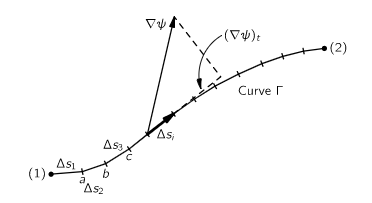
\includegraphics[scale = 0.6]{math prelim/images_math prelim/line integral}
    \caption{Line integral illustration}
    \label{Line int pic}
\end{figure}
\begin{equation}
	\Delta \vec{s}_{i} \to 0 \hspace{15mm} n \to \infty 
\end{equation}
We can then find write the summation of the transport equation applied to each individual segment as an integral, 
\begin{equation}
	\label{line integral def}
	T_{(2)} - T_{(1)} = \int_{(1)}^{(2)} \vec{\nabla} T \cdot d\vec{s}
\end{equation}
Physically, we can represent it as in the following figure. Each part of the summation, i.e $\vec{\nabla} T_{i} \cdot \Delta \vec{s}_{i}$ represents the projection of the grad of $T$ onto the segment $\Delta \vec{s}_{i}$. The above result is then defined as the \emph{line integral}. A similar concept can be extended when dealing with vector fields instead of scalar fields. Suppose that there is a vector field $\vec{h}$ that represents the heat flow per unit area coming out of a surface. If we are then interested in the amount of heat flow that is exiting the surface, we can then consider an elemental area $\Delta a$ just like we broke up the curve, $\psi$ into tiny straight segments. The heat flow coming out of the tiny element can then be represented as, 
\begin{equation}
	\label{elemental outflow}
	\text{Heat flow out of elemental area} = \vec{h}_{i} \cdot \vec{n}_{i} \Delta a_{i}
\end{equation}
From the above equation, we infer that for each elemental area, $\Delta a_{i}$ there is a corresponding vector $\vec{n}_{i}$ that is normal to the area. In addition, there is a corresponding vector $\vec{h}_{i}$ that represents the heat flow vector coming out of $\Delta a_{i}$, which might not be necessarily normal to $\Delta a_{i}$. If we then impose the condition that, 
% insert figure for surface integral
\begin{figure}[H]
    \centering
    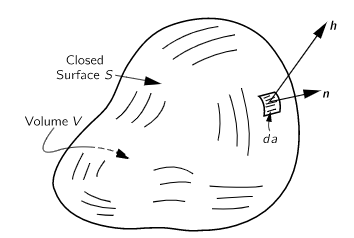
\includegraphics[scale = 0.6]{math prelim/images_math prelim/surface integral}
    \caption{Surface integral illustration}
    \label{Surface int pic}
\end{figure}
\begin{equation}
	\Delta a_{i} \to 0 
\end{equation}
We can write the summation of \autoref{elemental outflow} applied to all segments as an integral. 
\begin{equation}
	\frac{d Q_{out, S}}{dt} = \int_{S} \vec{h} \cdot \vec{n} da
\end{equation}
The above equation then refers to a \emph{surface integral}. 
\subsection{Gauss' Theorem}
Next, we can go on to write the relationship between the flux through a surface with flux through a volume. Consider the figure below. The flux through surface 1 can be written as: 
% insert figure for elemental cube
\begin{figure}[H]
    \centering
    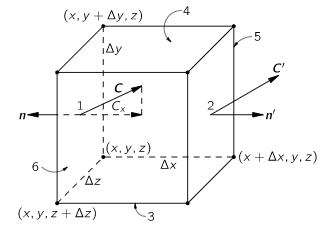
\includegraphics[scale = 0.6]{math prelim/images_math prelim/cube}
    \caption{Flux of $\vec{C}$ through elemental cube}
    \label{cube}
\end{figure}
\begin{equation}
	\text{Flux through (1)} = -C_{x}(1)\Delta y \Delta z
\end{equation}
On the other side, the flux through surface 2 can be written as: 
\begin{equation}
	\text{Flux through (2)} = -C_{x}(2)\Delta y \Delta z
\end{equation}
We then assume that this cube is very small, and that the following relationship would hold. 
\begin{equation}
	C_{x}(2) = C_{x}(1) + \frac{\partial C_{x}}{\partial x} \Delta x
\end{equation}
Which implies, 
\begin{align} 
	\text{Flux through (2)} &= -C_{x}(1)\Delta y \Delta z + \frac{\partial C_{x}}{\partial x} \Delta x \Delta y \Delta z\\
	\text{Total flux through (2) and (1)} &= -C_{x}(1)\Delta y \Delta z + \frac{\partial C_{x}}{\partial x} \Delta x \Delta y \Delta z -C_{x}(1)\Delta y \Delta z \\
	&= \frac{\partial C_{x}}{\partial x} \Delta V
\end{align}
A similar derivation can be performed for the flux through surfaces 3,4 and 5,6. We can then sum the total flux through all the surfaces as: 
\begin{align}
	\text{Total flux} &= \Big[ \frac{\partial C_{x}}{\partial x} + \frac{\partial C_{y}}{\partial y} + \frac{\partial C_{z}}{\partial z} \Big] \Delta V\\
	&= \vec{\nabla} \cdot \vec{C} \Delta V
\end{align}
Moving away from an elemental volume, larger volumes can be considered in a similar fashion by simply breaking up the large volume into many elemental volumes and applying the above result using integration. We get the following result: 
\begin{equation}
	\frac{d Q_{out, V}}{dt} = \int_{V} \vec{\nabla} \cdot \vec{C} dV
\end{equation}

From the previous theorem, we already know what the flux through a surface is by employing the use of surface integrals. We then have to notice that the flux through a volume is nothing but the flux through the surface that \emph{encloses} the volume. With this, we arrive at \emph{Gauss' theorem}. 
\begin{equation}
	\int_{S} \vec{C} \cdot \vec{n} da = \int_{V} \vec{\nabla} \cdot \vec{C} dV 
\end{equation}
\subsection{Circulation of a vector field and Stokes' theorem}
Consider the image below. The circulation of a vector field is then defined as the summation of the tangential components of the vector field along the closed loop. 
% insert image of circulation
\begin{figure}[H]
    \centering
    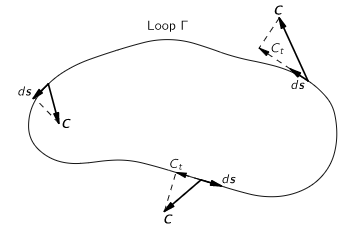
\includegraphics[scale = 0.6]{math prelim/images_math prelim/circulation}
    \caption{Circulation of $\vec{C}$ around $\Gamma$ visualised}
    \label{circ pic}
\end{figure}
\begin{equation}
	\text{Circulation of $\vec{C}$ around $\Gamma$} = \oint_{\Gamma} \vec{C} \cdot d\vec{s}
\end{equation}
As we have seen time and again, we can consider the circulation of a vector field around the boundary of a large surface by summing up the circulation around the boundary of elementary surfaces within the large surface in question. The circulation along of the edges of shared boundary would cancel out due to the opposing directions of circulation. Furthermore, if we constrain the elemental surfaces to be small enough, any curved surface will approximately be flat and taken as a square. From the figure below, we consider the circulation of vector field $\vec{C}$ around a small elemental square. 
% insert of figure of elemental square 
\begin{figure}[H]
    \centering
    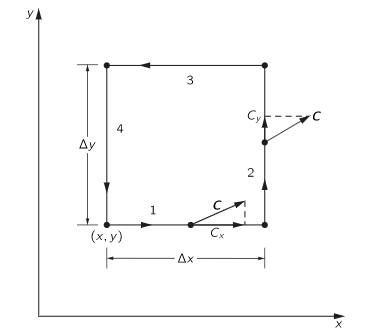
\includegraphics[scale = 0.6]{math prelim/images_math prelim/surface}
    \caption{Circulation of $\vec{C}$ around an elemental square surface}
    \label{stokes pic}
\end{figure}
It can also be assumed that the sides of the square is small enough such that the vector field does not change much along the length of a side. From the definition of circulation as discussed above, the circulation around this elemental square can be written as: 
\begin{equation}
	\label{circulation equation for elemental square}
	\oint_{\Gamma} \vec{C} \cdot d\vec{s} = C_{x}(1)\Delta x + C_{y}(2)\Delta y - C_{x}(3) \Delta x - C_{y}(4) \Delta y
\end{equation}
Note that the minus signs that arise are from the direction of circulation, which is positive in the anti-clockwise direction (right hand rule). We then can write the relationship between $C_{x}(1), C_{x}(3)$ and $C_{y}(2),C_{y}(4)$. 
\begin{align} 
	C_{x}(3) &= C_{x}(1) + \frac{\partial C_{x}}{\partial y}\Delta y\\
	C_{y}(2) &= C_{y}(4) + \frac{\partial C_{y}}{\partial x}\Delta x
\end{align}
Substituting the above relationships into \autoref{circulation equation for elemental square}, 
\begin{align}
	\oint_{\Gamma} \vec{C} \cdot d\vec{s} &= \frac{\partial C_{y}}{\partial x}\Delta x\Delta y - \frac{\partial C_{x}}{\partial y}\Delta y \Delta x\\
	&= \Big[ \frac{\partial C_{y}}{\partial x} - \frac{\partial C_{x}}{\partial y} \Big]\Delta a\\
	&= \Big[ \vec{\nabla} \times \vec{C} \Big]_{z}\Delta a
\end{align}
From the figure, we notice that the $z$-axis is nothing but the direction that is $\perp$ to the elemental surface. So, there is nothing special about the appearance of the $z$-coordinate of $\vec{\nabla} \times \vec{C}$ appearing in the circulation derivation. We can then present \emph{Stokes' theorem}, 
\begin{equation}
	\oint_{\Gamma} \vec{C} \cdot d\vec{s} = \int_{S} \Big[ \vec{\nabla} \times \vec{C} \Big]_{n}da
\end{equation}
















































